\documentclass[12pt, a4paper, oneside]{ctexart}
\usepackage{graphicx}
\usepackage{tikz}

\title{Uniswap简明导论}
\author{Splendor White}
\date{\today}

\begin{document}

\maketitle

\section{简介}

Uniswap 是以太坊区块链上的一个去中心化交易所。它既表现出与传统中心化交易所不同的特性,又是去中心化交易所的典型代表。了解其基本运行机制,是认识去中心化金融的基础。

与传统的中心化交易所不同,Uniswap 的交易不需要订单簿,而是由自动做市商根据恒定乘积公式对流动性池进行动态调整,满足交易者的交易需求。流动性提供者可以向流动性池中添加流动性,降低交易者的滑点,并按照份额赚取流动性费用。

Uniswap 是一个不断发展的交易协议。在 Uniswap V2 中,任意交易对、安全的价格预言机、闪电兑等功能得以实现。在 Uniswap V3 中,集中流动性的引入大大提高了资金利用率。在即将上线的 Uniswap V4 中,挂钩、单例、闪电记账等新元素使得合约可以更加灵活地定制化。

\section{订单簿与自动做市商}

\subsection{订单簿}

在传统的金融交易过程中,一部分买者和卖者需要在一个公共的\textbf{订单簿}(Order Book)上给出自己的买进报价(Bid)或卖出报价(Ask),这类交易者被称为挂单者(Maker)。其他的买者和卖者可以在订单簿中找到自己心仪的报价,并付给相应的商品或货币,从而完成交易,这类交易者被称为吃单者(Taker)。如图1所示。

\begin{figure}[htbp]
    \centering
    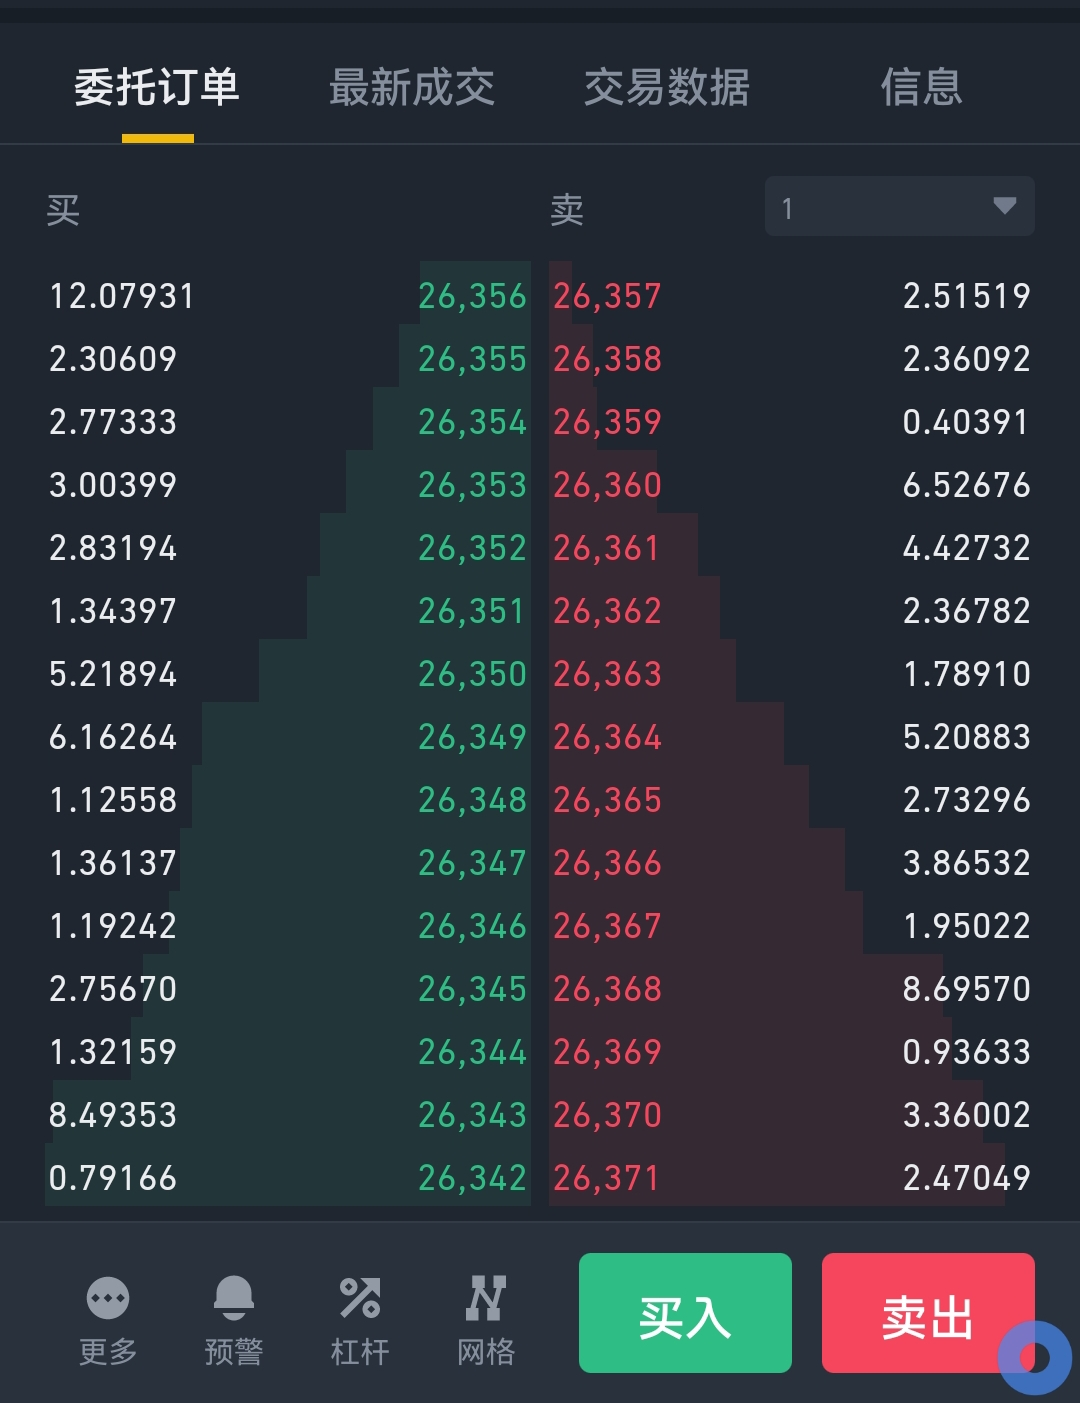
\includegraphics[width=8cm]{订单簿示意图.jpg}
    \caption{订单簿示意图}
\end{figure}

这种交易方式能够确定每一笔订单的成交价格和成交数量,并使得市场深度一目了然。但其流动性是不稳定的,市场深度有时大有时小。而且,由于所有的挂单信息都是公开的,市场操纵者可以根据这些信息使用一定数量的资金来将价格瞬间调整到自己想要的水平。

在订单簿模式下,如果挂单者寥寥无几,成交就会变得异常困难。有没有办法让交易者(无论是买者还是卖者)都能在任意时刻轻松成交呢?自动做市商实现了这一点

\subsection{自助售货机}

为了理解自动做市商,我们可以先以自助售货机作为一个例子。

考虑一个 24 小时不停工作的可口可乐售货机,里面存放着若干瓶可口可乐和一些零钱。当你想要购买一瓶可乐的时候,你需要将钱放入售货机中,然后售货机就会弹出一瓶可乐。现在,让我们将这个模式推广一下——假设你用某种手段(e.g. 走私或者自制)搞来原装的可口可乐,来到自助售货机面前,希望将可乐卖成零钱。你需要做的就是将可口可乐放入自助售货机中,然后售货机就会将相应的零钱付给你。这样,我们就拥有了一个可口可乐交易所。

假设最开始机器中有 $x_0$ 瓶可乐与 $y_0$ 枚一元硬币,并约定一瓶可乐的价格是 3 元。经过若干次交易之后,机器中有 $x$ 瓶可乐与 $y$ 枚一元硬币。很显然,我们有下面的恒等式:

\begin{equation}
    3x + y = 3x_0 + y_0
\end{equation}

这意味着,\textbf{留在机器中的可乐价值与硬币价值的总和是一个定值},我们设 $k=3x_0+y_0$ ,于是有

\begin{equation}
    3x + y = k
\end{equation}

将这个式子化为 $y = -3x + k$ ,并画出其函数图像,我们得到一个一次函数(如图2所示)。

\begin{figure}[htbp]
    \centering
    \begin{tikzpicture}
        \draw[-latex] (0,0) -- (2.5,0) node[right] {$x$};
        \draw[-latex] (0,0) -- (0,4) node[above] {$y$};
        \draw[domain=0:1, thick, red] plot (\x, {-\x*3+3});
        \node[left] at (0,3) {$k$};
    \end{tikzpicture}
    \caption{可乐交易所}
\end{figure}

然而,我们可能会遇到这样的窘境:我们一次性想要买的可乐太多了,机器里的可乐根本不够;或者我们一次性想要卖的可乐太多了,机器里的钱根本不够。这其实就是流动性问题。

解决这个问题的办法是显然的,我们只需要在机器中额外地投放更多的可乐或硬币即可。投放更多的可乐与硬币,使得机器的总价值从 $k$ 变为 $k'$ ,其中 $k' > k$ 。于是恒等式 (2) 变为

\begin{equation}
    3x + y = k'
\end{equation}

相应的函数图像变为

\begin{figure}[htbp]
    \centering
    \begin{tikzpicture}
        \draw[-latex] (0,0) -- (4,0) node[right] {$x$};
        \draw[-latex] (0,0) -- (0,7) node[above] {$y$};
        \draw[domain=0:1, thick, red] plot (\x, {-\x*3+3});
        \node[left] at (0,3) {$k$};
        \draw[domain=0:2, thick, blue] plot (\x, {-\x*3+6});
        \node[left] at (0,6) {$k'$};
        \draw[->] (0.5,1.5) -- (1.3,2);
    \end{tikzpicture}
    \caption{添加流动性后的可乐交易所}
\end{figure}



\end{document}

